\documentclass[conference]{IEEEtran}[10]
\IEEEoverridecommandlockouts
\usepackage{cite}
\usepackage{amsmath,amssymb,amsfonts}
\usepackage{graphicx}
\usepackage{textcomp}
\usepackage{xcolor}
\usepackage{float}
\usepackage{anyfontsize}
\usepackage {hyperref}
\usepackage{authblk}
\begin{document}
\title{House Rent Prediction using polynomial and linear regression}
\author[1]{ Amit Roy
}
\affil[1]{ID: 2017-3-60-021
}

\author[2]{ Sirajum Maria Muna
}
\affil[2]{ID: 2017-3-60-020
}

\author[3]{ Shekhor Chandra Saha
}
\affil[3]{ID: 2017-3-60-025
}

\author[4]{ Saniat Injam
}
\affil[4]{ID: 2017-3-60-093
}

\maketitle
\IEEEpubidadjcol
\section{INTRODUCTION}
\subsection{1.1 Objectives}
With the mass growth of population around the world, it has become a challenge to provide accommodation for the people. As well as the growth of population the housing prices are also becoming high. For this reason, people opting for house renting as, owning a house seem like a dream like to some people. In this project our aim is to find house rent for a certain area in different cities. We are using a combination of linear regression and polynomial regression to predict house rent prices. 
\subsection{1.2 Motivation}
As we live in a third world country, also a over populated one, finding a good place to live a life peacefully is not easy. Along with ourselves, we want to secure a good future for our next generations. But money is always a problem. So, in this project we are motivated by this idea and tried to do a better approach, so that, it can help us by predicting the rental price to make us learn, on which area has better facilities in our suited budget. If anyone wants to further invest on real estates, this approach can help them. Also, it can be the parameter to signify one area’s demand.
\subsection*{1.3 Existing works}
Several machine learning algorithms have been used in the past years in this field. A study has been done in Fairfax County, Virginia using several machine learning algorithms like Naïve Bayes, Ripper, Decision Tree, Adaboost etc. to predict the house prices.1
Ridge and Lasso Linear regression is being used in the area of Ames and Lowa. 2
Also, Hybrid Linear Regression is being used by combining Ridge and Lasso along with Gradient Boosting combination to find more accurate predicted values with higher accuracy. 3
By all these studies, what we have done till now, we have seen using hybrid machine learning algorithms gives better result than only one algorithm. Also, regression is a common classifier in that field. So, we have chosen to work on this part in our project.
\subsection*{1.4 Necessity}
As we have discussed in the motivation part, house rent prediction work can be used in daily basis to predict rental prices. In house rental dataset there can be several fractional values as well as non-numerical values. So, using regression is the safe option, as it works with fractional values and the non-numeric values can be pre-processed before the algorithm runs. Being less time consumption is another plus point of regression. The rental price prediction approach can ease many  manual work and gives people high efficient work facilities. 

\section{METHODOLOGY}
\begin{figure}[H]
\centering
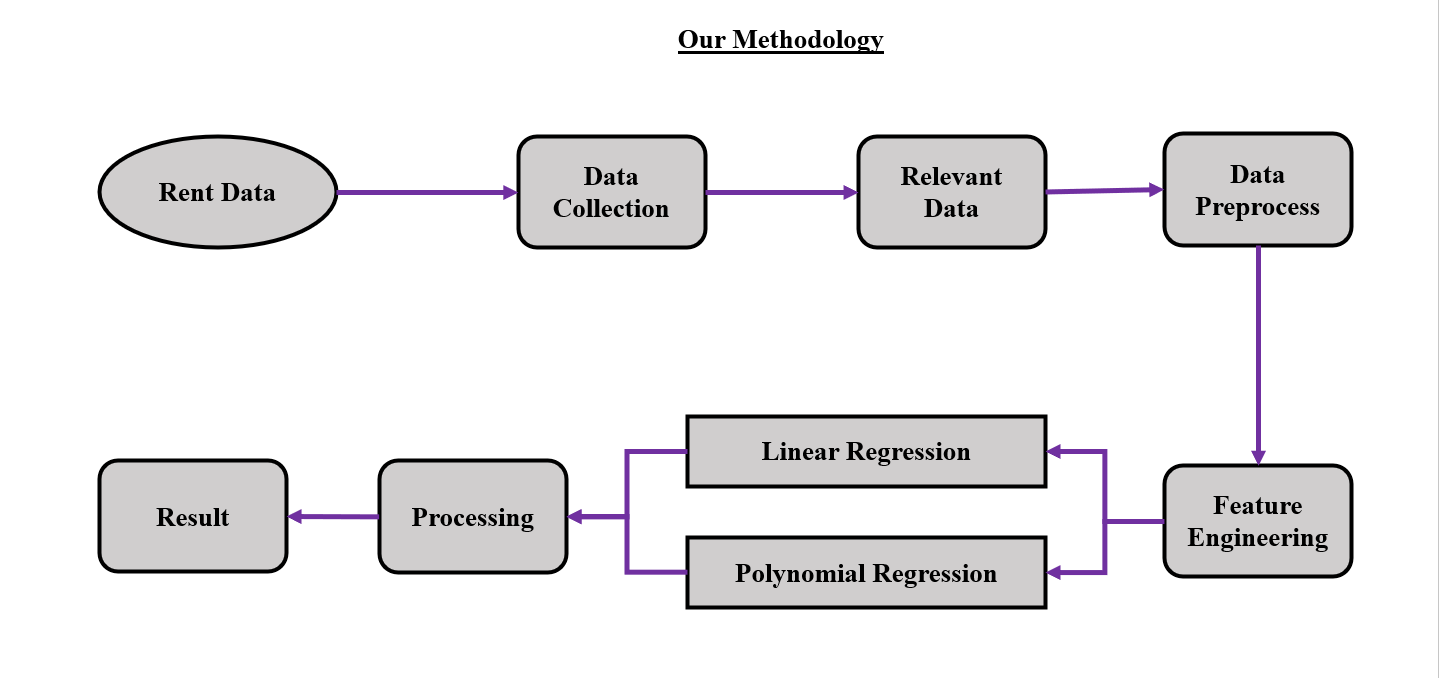
\includegraphics[scale=0.2]{methodology}
\caption{ Diagram of our proposed model}
\end{figure}
\section{IMPLEMENTATION}
\subsection{Model development}
We have worked with 2 types of regression: linear and polynomial regression and will estimate the accuracy between the models. In our final dataset we have 193011 rows and 21 columns. The dataset is divided according to the attributes in two sets: one is independent set, and another is dependent set
\end{document}